\documentclass{thesis}

% Writing Tips ================================================================
% Your research question should always be kept in mind. Write with it.
% https://moodle.gla.ac.uk/pluginfile.php/2676039/mod_resource/content/1/PRISMA%20statement.pdf
% https://moodle.gla.ac.uk/course/view.php?id=12843&section=7

% Style Guide =================================================================
% https://moodle.gla.ac.uk/pluginfile.php/4294369/mod_resource/content/1/ODL%20Project%20Style%20Guide.pdf
% The page limit is 25-30 for main content.

\usepackage{pdfpages}

\begin{document}

% Metadata ====================================================================

\title{Regressing Litter on Deprivation in Glasgow City with Object Detection}
\author{Gary Blackwood}
\date{\today}
\maketitle

% Abstract ====================================================================
% https://www.scribbr.com/dissertation/abstract/
% https://www.discoverphds.com/advice/doing/abstract-for-a-dissertation-or-thesis
% https://mantex.co.uk/how-to-write-a-thesis-abstract/

\begin{abstract}
    \todo{Abstract -- An executive summary of roughly 500 words.}
\end{abstract}

% Acknowledgements ============================================================
% https://www.discoverphds.com/advice/doing/acknowledgements-for-thesis-and-dissertations
% https://prothesiswriter.com/blog/how-to-write-an-acknowledgement-for-a-thesis

\chapter*{Acknowledgements}
\todo{}

% List of Figures and List of Tables ==========================================

\listoffigures
\listoftables

%==============================================================================

\tableofcontents

% Introduction ================================================================
% Background to research
% Research question
% Research aims
% Scope of research
% Importance of research
% Assumptions

\chapter{Introduction}
\pagenumbering{arabic} % Don't remove this!

The Scottish city of Glasgow was home to the 26th UN Climate Change Conference during the month of November 2021. Known as COP26, the gathering of world leaders, with thousands of delegates and diplomats in tow, was thought to be humanities last chance to commit to the changes necessary to keep global temperatures from rising past the limit of 1.5 degrees Celsius above pre-industrial levels. Breaking through this threshold would see catastrophic outcomes such as the increased intensity and frequency of droughts and floods\cite{impacts-of-15}.

This rightful focus on the global climate emergency overshadowed another environmental problem. One which, for Glasgow City at least, is at its worst state in years\cite{tackle-litter} -- the amount of litter on its streets.

According to a recent study by Keep Scotland Beautiful, the issue of litter creates the most public outcry\cite{household-survey-2019} and is an important indicator of overall environmental quality. Unfortunately, the study found that since 2016, the state of our public spaces has been in decline. None more so than in the most deprived areas of the country where the number of significantly littered sites has more than doubled since 2014.

Littering behaviour is strongly affected by the social context in which it occurs\cite{littering-behaviour}. Research by Zero Waste Scotland found that in addition to personal factors such as age and gender, social factors influenced the prevalence of litter. If individuals in an area deem it socially acceptable, it is more likely to occur. 

Why is there more litter in the most deprived areas? The socioeconomic problems that come with deprivation may be the answer. If the local population have more pressing troubles to worry about, they may care less about the environmental impacts of litter.

The Scottish Government seeks to understand the circumstances  surrounding deprived communities in order to make effective policy making decisions. If there are links between deprivation and littering, there may be the potential for the improvement of one issue to improve the other. Tackling litter by creating a fairer society is an exciting thought, but first we must discover the links between litter and deprivation.

This study aimed to identify the relationship between the key indicators of deprivation in areas of Glasgow City and the amount of litter on its streets. To this end, the Poisson and Negative Binomial regression models for count data were employed. The ambition was to discover areas of focus that could reduce littering if improved.

Secondary to this aspiration, it was of interest to discover if an automated approach to counting litter on a city scale could be achieved using deep learning object detection methods. Thus far, local organisations have had to perform manual audits to collect such data. Any improvement to this process would be a welcome step towards a cleaner world.

% Literature Review ===========================================================
% https://moodle.gla.ac.uk/mod/resource/view.php?id=841188
% demonstrates a familiarity with a body of knowledge and establishes the credibility of your work;
% summarises prior research and says how your project is linked to it;
% integrates and summarises what is known about a subject;
% demonstrates that you have learnt from others and that your research is a starting point for new ideas.

\chapter{Literature Review}

\section{Object Detection}

\subsection{CNN}

Convolutional Neural Network object detectors use supervised learning and generally consist of two components; a CNN-based backbone that is used for feature extraction, and a head that is used to predict the class and bounding box for an object. In recent years, state-of-art models have begun to insert layers in-between the backbone and head to form a third component known as the neck.

Existing Backbones are typically used for their proven feature extraction capabilities on classification problems. Rather than redesign custom networks, researchers will fine-tune the backbone to increase its suitability to the task at hand. Often used backbones include ResNet, VGG, and CSPDarknet53\cite{zhu2021tphyolov5}.

The purpose of the neck is to improve upon the features provided by the backbone. Usually consisting of several bottom-up and top-down paths, the neck reprocesses the backbone's features at different stages with the goal of aggregating them in preparation for the detection in the head.

The responsibility of detecting the location and category of an object falls upon the head. It takes the features extracted from the preceding layer's classification network and turns them into a prediction. 

There are generally two kinds of object detectors: one-stage and two-stage. Two-stage detectors have separate phases for bounding box and class predictions and for many years was the most popular method. The R-CNN series of detectors\cite{frcnn} is a representative example. One-stage detectors, like YOLO, accept the trade-off of faster detection for lower accuracy by performing bounding box and class prediction at the same time.

\subsection{Evaluation}

Evaluating object detection is challenging as it involves performing classification to determine whether or not an object exists, and localisation to determine the location of that object. 

A typical data set will contain a non-uniform distribution of many classes. If a a simple accuracy based metric was used for evaluation a biased result would be produced. For this reason, the mean average precision (mAP) metric was created.

The mean average precision (mAP) quantifies the performance of an object detector across all test images, classes, and at different confidence thresholds.

To calculate mAP and measure correctness, overlap between the predicted bounding box and ground truth box is measured using its intersection over union (IoU). 

\begin{equation}
    IoU = \frac{Area of Overlap}{Area of Union}
\end{equation}

Precision and recall measures are calculated for a class using the IoU value for many IoU thresholds. If the IoU value is greater than the threshold, the prediction is treated as a true positive. Otherwise, it is considered a false positive. The precision measures the percentage of correct predictions made and the recall measures the percentage of positives that were correctly identified. An object detector can trade-off precision for recall and vice-versa by adjusting the confidence level needed to make a prediction.

Precision-recall curves are constructed by setting the IoU threshold at varying levels of difficulty e.g. from 0.5--0.95 in increments of 0.05. The average precision (AP) is calculated individually for each class, before finally being averaged across all classes to produce the evaluation metric.

As a complement to mAP, the F1 metric combines the precision and recall measures to find the ideal confidence threshold which maximises them both. Similarly,
the area under the curve (AUC) metric integrates the amount of plot that falls underneath the precision-recall curve.

Most state-of-art object detectors publish their results using the mAP evaluation of well known challenges such as COCO\cite{lin2015microsoft} and Pascal VOC\cite{Everingham15}. However, as it depends on a subjective confidence level there can be a large gap between it and the actual accuracy\cite{Peng2021}. Researchers have studied ways to address this for classification problems by calibrating the confidence level beforehand\cite{guo2017calibration}, but material for object detection is minimal due to its complexity.


\subsection{YOLO}

You Only Look Once (YOLOv1), a neural network based approach to object detection, was first published in a 2015 paper titled \textit{You Only Look Once: Unified, Real-Time Object Detection}. The paper describes how the authors combined a previously multi-step object detection process into a single neural network that performs classification and bounding box detection.

With a unified structure facilitating end-to-end optimisations on detection performance, the network is able to outperform existing methods such as R-CNN in terms of accuracy and speed.\cite{yolov1}. In contrast to detection systems that re-purpose classifiers, YOLO re-frames the task into a regression problem that outputs class probabilities and bounding boxes by inspecting each image only a single time. 

The motivation of the authors was for the detector to literally "only look once", such that a single neural network would produce vectors of object predictions when given an input image.

The researchers found that training on full images brought about several benefits. With the ability to view the entire image, the model includes contextual information that competing methods are missing\cite{frcnn}. The result is a model that makes less than half the number of background errors compared to Fast R-CNN\cite{yolov1}.

As a result of its simplicity, the model is extremely fast because it only has to run its singular convolutional neural network on new images. With speeds up to 150 frames per second\cite{yolov1}, the model is promising for real-time applications.

It was found that the model performed well when applied to new domains because of its ability to learn generalisable representations of the objects it is detecting. However, it did not match the best performing detectors in terms of accuracy due to its difficulty in identifying the precise location of small objects.

In the follow up paper, \textit{YOLO9000: Better, Faster, Stronger}, an improved version of the model is described. Known as YOLOv2, it addresses a number of its predecessors shortcomings. The model's poor recall and aforementioned localisation errors are improved by modifications including the introduction of batch normalization and increasing the resolution of the classifier\cite{yolo2}.

\textit{YOLOv3: An Incremental Improvement} presents further advancements that produced a bigger, but more accurate network. The paper highlights that although previous iterations of the model struggled with small objects, the third version reverses this trend. The trade-off however, was slightly worse performance on objects of medium and large size\cite{yolo3}.

The penultimate iteration of the model (YOLOv4) achieves state-of-the-art results by combining universal detection features: Weighted-Residual-Connections, Cross-Stage-Partial-connections, Cross mini-Batch Normalization, Self-adversarial training, and Mish-activation\cite{yolov4}. The publication highlights how the majority of accurate detectors do not facilitate real-time operation before explaining how this problem is overcome by creating a convolutional neural network for which training requires only a single conventional graphics processing unit with 8--16 GB of memory. The result is a model which is faster, in terms of frames per second, and more accurate, using the MS COCO AP metric, than all competition.

YOLOv5 is the latest object detector of its kind and it offers different pre-trained models including YOLOv5n, YOLOv5s, YOLOV5m, YOLOv5l and YOLOV5x. From smallest and fastest to largest and slowest respectively, each has a domain in which it is most appropriate. For example, the small YOLOv5s model can deployed on mobile devices as it has significantly less parameters (millions) and requires considerably less GPU memory to train and run than the larger models\cite{yolov5}.

The architecture consists of a CSPDarknet53 backbone with an SPP layer, and a PANet neck that is followed by a YOLO detection head\cite{yolov1}. Bags of freebies and specials are implemented as optimisations to increase accuracy with a minimal increase in inference cost\cite{yolov4}.

\subsection{Faster R-CNN}

Leading detection performance was achieved on the Pascal VOC challenge data set by combining region proposals with CNNs in a method known as Regions with CNN features. R-CNN used a multi-stage pipeline that extracted features, tuned the network using log less, and trained SVMs before finally fitting bounding-box regressors\cite{rcnn}. The complexity of this architecture resulted in large space and time requirements for training. Efforts were made to reduce these requirements by sharing computation using Spatial Pyramid Pooling Networks. SPPnets compute classifierd object proposals using a feature vector that has been extracted from a shared feature map. It reduced training time by a factor of three as a result of its faster proposal feature extraction\cite{he2015spatial}.

In a follow up to his original paper, the author proposed Fast R-CNN as a method that fixed the disadvantages of R-CNN while simultaneously improving its accuracy and speed\cite{fast-rcnn}. Building from this, the Faster R-CNN method made further improvements to reduce the proposal generation computational complexity. By sharing the same convolutional layers for the detector and RPN, the method was able to support passing an image through the network only once\cite{frcnn}.

\begin{figure}[h]
    \centering
    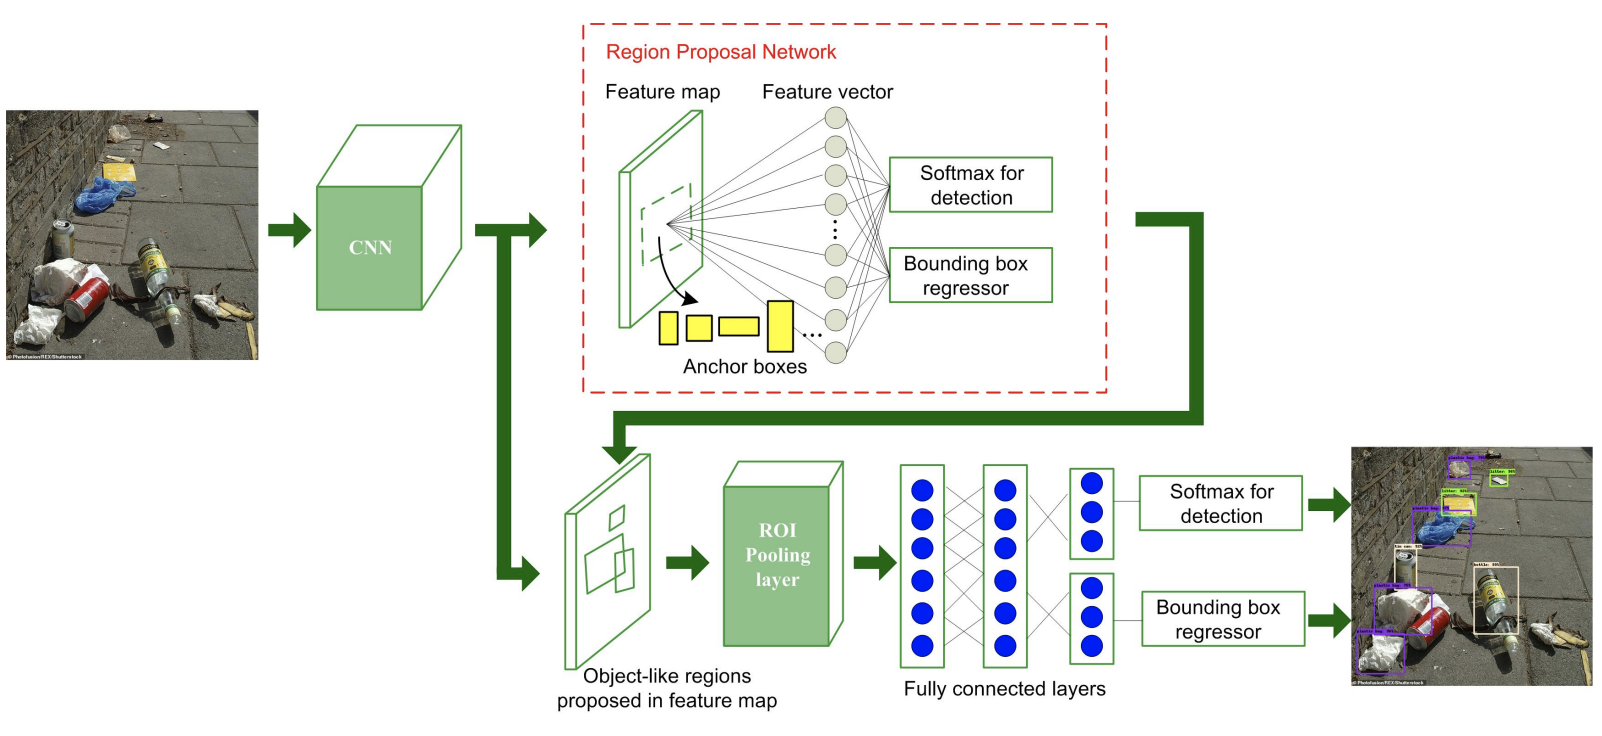
\includegraphics[scale=0.5]{images/faster-rcnn-architecture.png}
    \caption{The architecture of Faster R-CNN\cite{smart-street}.}
    \label{fig:faster-rcnn-architecture}
\end{figure}

Figure \ref{fig:faster-rcnn-architecture} illustrates how Faster R-CNN uses layers known as Region Proposal Networks (RPN) to generate feature maps which are turned into object region proposals. The proposals are projected onto the feature map and objects are detected by classifying the proposals. Now a one-stage detector with a single network, Faster R-CNN, like YOLO\cite{yolov1}, can be trained end-to-end and optimised for detection performance.

\subsection{Litter}

Despite the availability of large data sets such as COCO\cite{lin2015microsoft}, litter is underrepresented due to its geographic and material variation. The Trash Annotations In Context (TACO) initiative aims to tackle this problem with the goal of improving autonomous litter monitoring systems\cite{DBLP:journals/corr/abs-2003-06975}. In its paper, the TACO researchers describe how it can often often be impossible to distinguish between different types of litter due to the small size of the objects and the resolution of the images. Cigarettes, one of the most commonly littered objects, mostly covered an area less than 64x64 pixels in size. This issue compounds with the lack of available data, which they attempt to address using augmentation and transplantation techniques. A Mask R-CNN model was trained, but the lack of annotated images and difficulty detecting small objects significantly impacted the resulting AP performance.

A Clean Europe Network summit meeting\footnote{https://cleaneuropenetwork.eu/en/measuring-litter/aus} concluded that a lack of data is contributing to the difficulty in addressing the environmental issues caused by urban littering. Cities throughout the world are assessing urban cleanliness by means of human audit. Without a practical approach to measuring an index of cleanliness, it will be challenging to properly manage the problem. 

Researchers in Spain proposed a cleanliness index for the city of Granada\cite{sevilla}. As part of its definition litter was weighted based on its classification, with larger objects assigned higher weights. The study used data that was manually collected by humans and provided by the organisation responsible for cleaning the city.

Attempts to quantify litter using automated object detection have been made\cite{cvstreets}. However, the lack of available data forced the researchers to manually collect and annotate images. A camera was attached to a vehicle and placed at a height of two to three meters from the ground. This limited the litter detection to objects within the immediate vicinity of the vehicle. In the paper, it is highlighted that no prior work has been undertaken to develop such an automated approach.

Efforts have also been made to automate the data collection process. Researchers in India have used the Bing Image Search API\footnote{https://www.microsoft.com/cognitive-services/en-us/bing-image-search-api} to gather a large and diverse set of 2561 images that could be used to train a CNN for detecting litter\cite{Mittal2016SpotGarbageSA}. They provide an Android mobile application that can be used by citizens to report litter in their communities. The approach focused on segmenting areas of an images taken by mobile phones, rather than the quantification of litter itself. In their paper, the authors describe how they utilised a pre-trained AlexNet\cite{NIPS2012_c399862d} model to obtain a 90.06\% specificity and 83.96\% sensitivity.

\section{Regression}

The inference of count data involves estimating the unknown parameters of a given probability distribution. The distribution models the number of occurrences of an event, such as train accidents in a given year, or a rate, such as the quantity of litter in a given area.

\subsection{Poisson}

The benchmark parametric model for count data is the Poisson distribution\cite{cameron_trivedi_2013}. Shown in equation \ref{eq:poisson-model}, the model assumes that the response $Y$ follows the Poisson distribution and it is concerned with modelling the effects of explanatory variables on the response through the rate parameter $\mu$. 

\begin{equation}
    E(Y_i) = \mu_i = n_i\theta_i = n_ie^{x_i^t\beta},\hspace{1em}Y_i = Poi(\mu_i)
    \label{eq:poisson-model}
\end{equation}

The unknown rate parameter $\mu$ is defined in terms of units of exposure, which is the length of time during which the events are recorded\cite{cameron_trivedi_2013}. Dependence on the explanatory variables is given by $\theta_i = n_ie^{x_i^t\beta}$ in which the $i$th covariate pattern is explained for exposure $n_i$.

The corresponding link function with offset $\log{n_i}$ is given by:

\begin{equation}
    \log{\mu_i} = \log{n_i} + x_i^t\beta
\end{equation}

The mean and variance of $Y \sim Poi(\mu)$ are both $\mu$ and the probability mass function for the distribution is given in equation \ref{eq:possion-pmf}. 

\begin{equation}
f(y) = \frac{\mu^ye^{-\mu}}{y!},\hspace{1em}y = 0, 1, 2,...
\label{eq:possion-pmf}
\end{equation}

This equality is known as the \textit{equidispersion} property of the Poisson and it is frequently not the case for real-world data. \textit{Overdispersion} is said to occur if the mean exceeds the variance. Similarly, \textit{underdispersion} presents itself if the variance is less than the mean. When data exhibit this property, it needs to be accounted for so that statistical inferences are valid\cite{understanding-poisson}.

Poisson regression models have been applied in many domains including health, finance and manufacturing. In 1992, the number of defects per area in a manufacturing process at the AT\&T Bell Laboratories was studied\cite{defects}. The researchers used the zero-inflated variant of the model to identify the set of conditions under which the mean number of defects was lowest.

\subsection{Negative Binomial}

Violations of the equidispersion property of the Poisson regression model can be dealt with by assuming a negative binomial distribution for the response $Y$, which allows for variances that are not equal to the mean.

The model form is the same as the Poisson and it introduces a new unknown variable $\alpha$ with density:

\begin{equation}
    f(y|\mu,\alpha) = \frac{\Gamma(y + \alpha^{-1})}{\Gamma(y+1)\Gamma(\alpha^{-1})}(\frac{\alpha^{-1}}{\alpha^{-1} + \mu})^{\alpha^{-1}}(\frac{\mu}{\alpha^{-1} + \mu})^y,\hspace{1em}\alpha\ge 0, y=0,1,2,...
\end{equation}

Both $\mu$ and $\alpha$ are estimated during model fitting. It has been suggested that $\alpha$ should be chosen such that the Pearson or deviance static is equal to $n - k$\cite{cameron_trivedi_2013}.

The model reduces to the Poisson if $\alpha = 0$ as it is used to explain the variance which is $Var(Y_i) = \mu_i + \alpha\mu_i^2$ for the NB2 model: the most common implementation of the negative binomial\cite{cameron_trivedi_2013}. This formulation is popular because it allows the modelling of Poisson heterogeneity using a gamma distribution\cite{ncss-neg-bin}.

% Data ========================================================================
% Data summary
% Data collection
% Ethical considerations

\chapter{Data}

The data for the study was collected from three independent sources.

\section{Scottish Index of Multiple Deprivation}

The Scottish Index of Multiple Deprivation (SIMD) is a tool for identifying the places in Scotland where people are experiencing disadvantage across different aspects of their lives \cite{simd}. Published by the Scottish Government, it provides a relative measure of deprivation across many small areas of the country.

The data are a collection of 6,976 data zones which represent areas with roughly equal populations of 700 -- 800 people. Each data zone has over 30 deprivation indicators such as crime rate, unemployment rate, and pupil attainment. By combining these indicators into a single index, the data zones are ranked relative to one another, from 1 -- 6,976, where rank 1 is the most deprived area in the country. In total, seven aspects of deprivation are combined: Income, Employment, Health, Education, skills and training, Geographic access to services, Crime, and Housing.

For the purposes of the study, the subset of data zones located in the Glasgow City council area was obtained, resulting in a collection of 746 data zones with associated deprivation indicators described in \ref{table:simd-deprivation-indicators}.

A revised version of the January 2020 publication was used for the study, in which the income domain and overall rankings were updated as a result of an error in the original data provided by the Department for Work and Pensions\footnote{https://www.gov.scot/publications/scottish-index-of-multiple-deprivation-2020v2-revision-notice}.

\subsection*{Missing Data}

A total of 137 missing indicator values were discovered in the data for Glasgow City. Indicated by a '*' character, the missing value is used when a value cannot be determined, or if the value has been suppressed for disclosure control where small numbers are involved.

To maintain as much information as possible in the small data set, missing values were imputed as the mean of the observed values.

\subsection*{Litter Response}

In order to answer the questions of interest, the amount of litter in each Glasgow City data zone was quantified and added to the SIMD data set as integer counts. The object detection methods used to achieve the creation of this response variable are  described in chapter \ref{chapter:methods}.

\begin{table}[ht!]
    \centering
    \begin{tabular}{||l p{100mm}||} 
     \hline
     \textbf{Indicator} & \textbf{Description} \\ [0.5ex] 
     \hline\hline
     Data\_Zone & Data zone name (string) \\
     Intermediate\_Zone & Intermediate zone name (string) \\
     Council\_area & Council area name (string)  \\
     Total\_population & Area population estimate (integer) \\
     Working\_age\_population & Area working age population estimate using state pension age (integer) \\
     Income\_rate & Percentage of people who are income deprived \\
     Employment\_rate & Percentage of people who are employment deprived \\
     Employment\_count & Number of people who are employment deprived (integer) \\
     CIF & Comparative illness factor (standardised ratio\footnotemark) \\
     ALCOHOL & Hospital stays related to alcohol use (standardised ratio) \\
     DRUG & Hospital stays related to drug use (standardised ratio) \\
     SMR & standardised mortality ratio (standardised ratio) \\
     DEPRESS & Percentage of population being prescribed drugs for anxiety, depression or psychosis \\
     LBWT & Percentage of live singleton births of low birth weight \\
     EMERG & Emergency stays in hospital (standardised ratio) \\
     Attendance & Percentage of school pupil attendance \\
     Attainment & Attainment score of school leavers (float) \\
     no\_qualifications & Working age of people with no qualifications (standardised ratio) \\
     not\_participating & Percentage of people aged 16 -- 19 not participating in education, employment or training \\
     University & Percentage of 17 -- 21 year olds entering university \\
     drive\_petrol & Average drive time to a petrol station in minutes (float) \\
     drive\_GP & Average drive time to a GP surgery in minutes (float) \\
     drive\_PO & Average drive time to a post office in minutes (float) \\
     drive\_primary & Average drive time to a primary school in minutes (float) \\
     drive\_retail & Average drive time to a retail centre in minutes (float) \\
     drive\_secondary & Average drive time to a secondary school in minutes (float) \\
     PT\_GP & Public transport travel time to a GP surgery in minutes (float) \\
     PT\_Post & Public transport travel time to a post office in minutes (float) \\
     PT\_retail & Public transport travel time to a retail centre in minutes (float) \\
     broadband & Percentage of premises without access to super fast broadband (float) \\
     crime\_count & Number of recorded crimes of violence, sexual offences, domestic housebreaking, vandalism, \newline drugs offences, and common assault (integer) \\
     crime\_rate & Number of recorded crimes of violence, sexual offences, domestic housebreaking, vandalism, \newline drugs offences, and common assault per 10,000 people (integer) \\
     overcrowded\_count & Number of people in households that are overcrowded (integer) \\
     nocentralheat\_count & Number of people in households without central heating (integer) \\
     overcrowded\_rate & Percentage of people in households that are overcrowded \\
     nocentralheat\_rate & Percentage of people in households without central heating \\ [1ex] 
     \hline
    \end{tabular}
    \caption{Description of the SIMD data zone deprivation indicators.}
    \label{table:simd-deprivation-indicators}
\end{table}

\footnotetext{A value of 100 is the Scotland average for a population with the same age and sex profile.}

\section{Google Street View Images}

To achieve a quantification of litter using object detection, thousands of images depicting the streets of Glasgow City were downloaded from the Google Maps Platform to be used as input to the  object detection models. 

Software\footnote{https://github.com/Garee/glasgow-litter} was developed to obtain the images using the Street View Static API\footnote{https://developers.google.com/maps/documentation/streetview/overview}. A random sample of 50 unique locations were generated within each data zone boundary and an image was downloaded at each.

A total of 37,300 images (50 for each data zone) were retrieved at the maximum resolution of 640x640 pixels at a pitch of 0 degrees with a 90 degree field of view from the source camera on the vehicle. Figure \ref{fig:street-view-image} is one such example.

\begin{figure}[h]
    \centering
    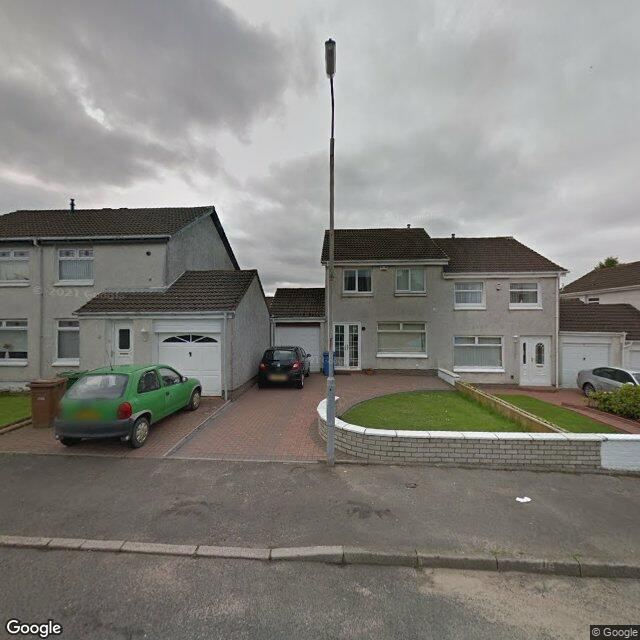
\includegraphics[scale=0.5]{images/street-view-image.jpg}
    \caption{A typical image of a Glasgow City street retrieved using the Google Maps Platform.}
    \label{fig:street-view-image}
\end{figure}

\subsection*{Privacy}

The images returned by Google have human faces and vehicle license plates automatically blurred to protect the privacy of individuals.

\section{Public Recycling Facility Locations}

The location and details of Glasgow City's 741 public recycling facilities were requested in JSON format from the public map\footnote{https://glasgowgis.maps.arcgis.com/apps/webappviewer/index.html?id=345f389a91ff4f1fa193b24df832fb05} hosted and maintained by Glasgow City Council.

Software was developed to count the number of facilities within each data zone boundary and add them to the SIMD data set as integers such that the count could be used as a potential explanatory variable.

% Methods =====================================================================
% Data Analysis

\chapter{Methods} \label{chapter:methods}
\todo{}

\section{Litter Detection}
\subsection{Yolov5}
\paragraph{Data Split}
\paragraph{Data Augmentation}
\paragraph{Transfer Learning}
\paragraph{Imbalanced Data Techniques}
\paragraph{Hyper-parameter Tuning}
\subsection{Faster RCNN}
\subsection{Model Selection}

\section{Regression}
\subsection{Exploratory Analysis}
\subsection{Poisson Regression}
\subsection{Negative Binomial Regression}
\subsection{Model Selection}

% Results =====================================================================
% https://moodle.gla.ac.uk/mod/resource/view.php?id=1517002

\chapter{Results}
\todo{}

\section{Litter Detection Accuracy}
\paragraph{Naive Classifier Comparison}
\paragraph{Generalisation To Other Locations}
\section{Deprivation Relationships}

% Discussion ==================================================================

\chapter{Discussion}
\todo{}

\section{Recommendations}
\section{Limitations and Future Work}
\section{Conclusion}

% Appendices ==================================================================

\begin{appendices}

\chapter{Source Code}
\todo{Appendices}

\end{appendices}

% Bibliography ================================================================

\bibliographystyle{alpha}
\renewcommand{\thechapter}{0} % Don't number the bibliography
\bibliography{thesis}

\end{document}
